\documentclass{article}%
\usepackage[T1]{fontenc}%
\usepackage[utf8]{inputenc}%
\usepackage{lmodern}%
\usepackage{textcomp}%
\usepackage{lastpage}%
\usepackage{authblk}%
\usepackage{graphicx}%
%
\title{Regulation of Histone Acetylation in the Nucleus by Sphingosine{-}1{-}Phosphate}%
\author{Monique Espinoza}%
\affil{Department of Oral and Maxillofacial Surgery, Hyogo College of Medicine, Nishinomiya, Hyogo 663{-}8501, Japan, Department of Genetics, Hyogo College of Medicine, Nishinomiya, Hyogo 663{-}8501, Japan}%
\date{01{-}01{-}2014}%
%
\begin{document}%
\normalsize%
\maketitle%
\section{Abstract}%
\label{sec:Abstract}%
A new study in RNA{-}seq was published in Science Translational Medicine: Ion Signaling. This paper was authored by Prof. Odysseas Petkas of Arezzo Professor of Molecular Cell Biology at the University of Washington and authors Miriam P. Sastry of UC Davis and Manuela Fiorillo of Universidad Autnoma de Mxico.\newline%
Analysis of RNA from two different regional gene transcription centers suggests that there is a genetic mechanism involved in enhancing new scarring in different kinds of collagen (a line of keratin cells) due to different forms of viral or host{-}mediated fibrosis. Two robust studies are available showing that this mechanism can be reduced in keratinocytes just by adding viral RNA, or RNA fusion RNA (RNA{-}I).\newline%
Both of the studies confirm the genetic role of viral RNA as a cellular trigger, says study lead author Amiliano Perez Quesada, PhD, from Universidad Autnoma de Mxico in Mxico. Together, these two genes appear to play a role in antiviral levels in cultured adult KL{-}4 KRASK cells from high{-}risk humans.\newline%
Authors specifically identify the active component of both viral and host{-}mediated infection as a combination of candidate RNAs, and the share of viral I RNA produced by the full genome. Viral HIV is implicated in cellular disease, but viral splicing is more controversial. In this study, participants who received viral factor VIII gene efflux prior to injection had significant protective effects against HIV infection, whereas those who received viral RNA insert/DNA replacement vector DNA injections had not significantly reduced their HIV baseline levels.\newline%
The full paper is available for free download at: http://press.sciencedirect.com/science/article/pii/S13338676124570522\newline%
All serogroups were isolated from phenotypic study groups, consisting of healthy and infected individuals in order to develop highly reproducible test tubes.\newline%
These studies offer a conceptually exciting outlook for drug discovery of new drug mechanisms. Merck, part of the Merck Research Laboratories, is internationally leading developer of biologics treatments for a wide range of diseases including cardiovascular, metabolic, immune and respiratory disorders and respiratory and inflammatory conditions, as well as autoimmune and cancer. Merck is also a leading manufacturer of pharmaceuticals.

%
\subsection{Image Analysis}%
\label{subsec:ImageAnalysis}%


\begin{figure}[h!]%
\centering%
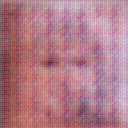
\includegraphics[width=150px]{500_fake_images/samples_5_72.png}%
\caption{A Black And White Photo Of A Black And White Cat}%
\end{figure}

%
\end{document}